\documentclass[11pt]{article}
\usepackage[utf8]{inputenc}
\usepackage[T1]{fontenc}
\usepackage[francais]{babel}
\usepackage[francais]{layout}
\usepackage{hyperref}
\usepackage{multicol}
\selectlanguage{french}

% NE PAS CHANGER !!
\ifx \public \undefined \def\public{enseignants} \fi
\usepackage[\public]{tps}
\usepackage{tikz}
\usepackage{amssymb}

\graphicspath{{imgs/}}

% Numéro du TP
\newcommand{\numtd}{03}
% Titre du TP
\newcommand{\titretd}{Integers and Bit Representation}
\def\tup#1{\langle #1\rangle}
\begin{document}
	
	\entete{\numtd}{\titretd}

\subsection*{Exercise 1 - Binary Operations}
The C language has bit manipulation mechanisms. For example, consider two variables $x$ and $y$ of type integer and the operator $\oplus$ (xor). We denote the $i$th bit of $x$ and $y$ by $x_i$ and $y_i$ respectively. The result of  $x \oplus y$ is the word $z$ such that $z_i = x_i \oplus y_i$.
The C operators are \verb+&+ (and), \verb+|+ (or), \verb+^+ (xor) and \verb+~+ (not). 

Do not confuse logical operators such as \verb+&&+, \verb+||+, etc. with operators for handling binary words. Note that \verb+4&2+ is 0, \verb+4&&2+ is 1.

Binary operations can be condensed. So \verb+x=x|2+ can be written \verb+x|=2+, and \verb+x=x^y+ can be written \verb+x^=y+. The language also provides the right shift operators $\gg$ or the left shift $\ll$.

\begin{enumerate}
	\item What does the following code do:
	\begin{verbatim}
		n & (n-1)
	\end{verbatim}
\begin{solution}
	Remove the least significant 1 (if $ n \ne 0 $). Equal to 0 if $ n = 0 $.
	\end{solution}

 \item In the following snippet $c$ and $n$ are integers.
\begin{verbatim}
	for (c = 0; n != 0; n &= (n-1)) c++;
\end{verbatim}
What value does $c$ take according to the values of $n$?
\begin{solution}
	Example with $n=5$.
	
	$c=0$ ; $n\ne0$ so \verb+n&(n-1)+ or \verb+5&4+, in binary \verb+101&100+,
	so $n=(100)_2$ and $c=1$.
	
	$n$ is greater than 0 so \verb+4&3+ or \verb+100&011+
	so $n=0$ and $c=2$.
	
	$c$ is the number of 1s in the binary representation of $n$.
\end{solution}
\end{enumerate}


We will study a method which efficiently counts the number of $1$s in a word of length $2^k$
(for a $k \geq 0)$, that is, in $\mathcal{O}(k)$ number of operations, assuming $2^k$ is the size of a register.
Let $l \leq k$ and $n$ be a word of length $2^k$. We denote by $l-block$ a block of $2^l$ consecutive bits in $n$, such that these blocks do not overlap . (For example, there are eight 2-blocks of length 4 in a 32-bit word.) The $l$-count of $n$ is the word of length $2^k$ such that each of its $l$ -blocks contains the number of 1's of the corresponding $l$-block in $n$. Trivially, any word equals its own 0-count. We try to produce the $k$-count of $n$.
In what follows, we will assume that $k = 5$, and suddenly we are working with 32-bit registers. The method is, however, easy to generalize.

\begin{enumerate} \addtocounter{enumi}{2}
	\item Find an operation that produces the 1-count of $n$ (in constant time).
	\begin{solution}
		In one copy of \verb-n-, we keep the bits in even positions,
		in another the bits in odd positions. This is done with the help of \emph{masking}. We know that for any bit $b$, $0\&b=0$ and $1\&b=b$. Hence, for the first copy, we \texttt{AND} the even positions with 1 (guarding) and the odd positions with 0 (masking). Similarly, for the second copy, we guard the odd positions and mask the even positions.  By shifting one of the copies,
		we can add all the blocks at the same time.
		
		\verb-((n & 0xaaaaaaaa) >> 1) + (n & 0x55555555)-
		
		Moreover, the additions are independent because any block is
		large enough to store the number of 1's of the original block. Hence, it is in constant time.
	\end{solution}
	\item Generalize and iterate this operation to calculate the 5-count of $n$.
	\begin{solution}
		We progressively generate the 1-count, 2-count, etc.
		
		\verb-n = ((n & 0xaaaaaaaa) >> 1) + (n & 0x55555555);-\\
		\verb-n = ((n & 0xcccccccc) >> 2) + (n & 0x33333333);-\\
		\verb-n = ((n & 0xf0f0f0f0) >> 4) + (n & 0x0f0f0f0f);-\\
		\verb-n = ((n & 0xff00ff00) >> 8) + (n & 0x00ff00ff);-\\
		\verb-n = ((n & 0xffff0000) >> 16) + (n & 0x0000ffff);-
	\end{solution}
\end{enumerate}

We work with 64-bit registers. Let $n=(stuvwxyz)_2$ be a byte, with $s$ the most significant bit and $z$ the least significant. 
\begin{enumerate} \addtocounter{enumi}{4} 
	\item What does the following C expression give?

\begin{verbatim}
	(n * 0x0202020202 & 0x010884422010) % 1023
\end{verbatim}

\begin{solution}
	This expression inverts the order of the bits. i.e. it gives $(zyxwvuts)_2$.
	\end{solution}
\end{enumerate}

\subsection*{Exercise 2 -  De Bruijn sequences}

In this part of the TD, we will develop an efficient method to count the number of trailing
zero bits in a given (unsigned) integer value $x$ such that $x > 0$. Equivalently, we can compute
the position of the least significant bit whose value is $1$. For example, if the binary representation of $x$ is $10110100$, then the bit we are looking for is the $1$ which is followed by the two final $0$s.
%Par exemple, si la représentation binaire de x est 10011000, alors le bit recherché est le 1 suivi par les trois zéros finaux. %Incidentally, one concrete application
%– when $x$ has $64$ bits – is to encode the positions of pieces on a chess board and iterate over
%these. Here however, we will simplify matters by assuming that $x$ has only $8$ bits.

An index in a bit string is identified from right to left starting at zero. E.g., for $x =
(10110100)_2$, the bits of $x$ at index $0$ and $1$ are $0$, and the bit with index $2$ is $1$. We present this method for $2^3=8$ bit words, but it can be generalized to $2^n$ bits for any $n>0$.

Given $x \in \mathbb{N}$ such that $0 < x < 2^8$, we will be interested in implementing a function
$\ell : \{1, \ldots, 2^8-1\} \rightarrow \{0, \ldots, 7\}$ such that $\ell(x)$ is equal to smallest index that is set to $1$ in
the binary representation of $x$. In the example above, we have $\ell(x) = 2$.

\begin{enumerate}
	\item Write a naive C function to solve this problem (skeleton below). 
	\begin{verbatim}
		unsigned int l (unsigned int x) { // we assume 0 < x < 256
			int result = 0;
			
			... //to be filled
			
			return result;
			
		}
	\end{verbatim}
	\begin{solution}
\begin{verbatim}
	unsigned int l (unsigned int x) { // we assume 0 < x < 256
		int result = 0;
		
		while (x & 1 == 0) {
			result++;
			x = x >> 1;
		}
		
		return result;
		
	}
\end{verbatim}
\end{solution}
\end{enumerate}

However, the running time of this function depends on the number of bits in $x$. We will
develop another algorithm has \emph{constant} running time, i.e. independent of the actual number
of zeros. To this end, we study \emph{de Bruijn} sequences. 

A de Bruijn sequence $s(n)$ of order
$n$ is a cyclic bit string such that every binary string of length $n$ occurs exactly once in $s$.
Cyclic means that once you reach the end of $s(n)$ you may continue at the beginning of $s(n)$.
For example, for $n = 2$ we can set $s(n) = 0011$ since $00, 01, 10$ and $11$ can all be found in
$s(n)$; in particular $10$ starts at index $0$ of s(n) and then continues at index $3$ of $s(n)$.


\begin{enumerate} \addtocounter{enumi}{1}
	\item Give a trivial lower bound for the minimal length of a de Bruijn sequence $s(n)$.
\end{enumerate}
\begin{solution}
	There are $ 2^n $ different words in $\mathcal{B}^n $.
	A trivial lower bound for a sequence $s$ is therefore
	of $ 2^n + (n-1) $, since each word in $ \mathcal{B}^n$
	must start at a position other than $s$ and must be followed
	by $n-1$ more bits.
\end{solution}

De Bruijn sequences can be obtained from paths in \emph{de Bruijn graphs}. The vertices of a de Bruijn graph of order $n$ are all bit strings of length $n$. There is a
directed edge between two vertices $b_1b_2 \cdots b_n$ and $c_1c_2 \cdots c_n$ if and only if $b_2 = c_1$, $b_3 = c_2, \ldots , b_n = c_{n-1}$.   

The figure~\ref{DeBruijnOrdre2} depicts the de Bruijn graph of order $2$.

\begin{figure}[h]
	\centering
	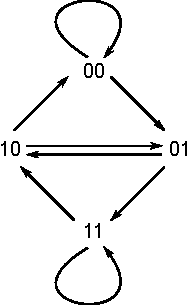
\includegraphics{order-2}
	\caption{\label{DeBruijnOrdre2}De Bruijn graph of order $2$.}
\end{figure}

\begin{enumerate}\addtocounter{enumi}{2}
	\item Draw the de Bruijn graph of order $3$.
\end{enumerate}
\begin{solution}
	\centerline{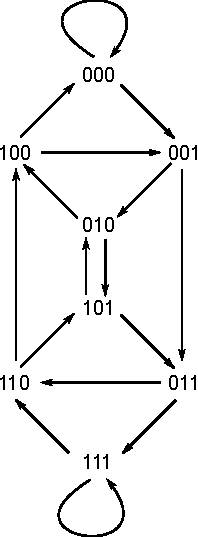
\includegraphics{order-3}}
\end{solution}


A de Bruijn sequence can be obtained from a de Bruijn graph by following
a \emph{Hamiltonian cycle} that starts and ends in the vertex $0 \cdots 0$. A Hamiltonian cycle is
a cycle that visits each vertex exactly once before returning to the starting vertex. For
instance, the only Hamiltonian cycle in the graph in the figure above is $00 \rightarrow 01 \rightarrow
11 \rightarrow 10 \rightarrow 00$. This cycle corresponds to the aforementioned de Bruijn sequence $0011$.
One can in fact prove that such a Hamiltonian cycle exists in every de Bruijn graph.% (see Bonus questions).

\begin{enumerate}\addtocounter{enumi}{3}
	\item Find two different de Bruijn sequences of order $3$ by following two different Hamiltonian paths in your de Bruijn graph of order $3$ starting in vertex $000$.
	
	\begin{solution}
		
		000 $\rightarrow$ 001 $\rightarrow$ 010 $\rightarrow$ 101 $\rightarrow$ 011
		$\rightarrow$ 111 $\rightarrow$ 110 $\rightarrow$ 100
		
		0001011100
		
		000 $\rightarrow$ 001 $\rightarrow$ 011 $\rightarrow$ 111 $\rightarrow$ 110
		$\rightarrow$ 101 $\rightarrow$ 010 $\rightarrow$ 100
		
		0001110100
		
	\end{solution}
	
	\item Choose a de Bruijn sequence $s(3)$ of order $3$ from the previous question and complete the following table:
	\begin{center}
		\begin{tabular}{ c | c }
			bit-string & 7- index in $s(3)$ \\
			\hline
			000 & 0 \\
			001 & \\
			010 & \\
			011 & \\
			100 & \\
			101 & \\
			110 & \\
			111 & \\
		\end{tabular}
	\end{center}

\begin{solution}
	
	Using the sequence 0001011100, we obtain the table below
	We observe that the right column is a permutation of $\{0,\ldots,7\}$.
	
	\begin{center}
		\begin{tabular}{ c | c }
			bit-string & index in $s$ \\
			\hline
			000 & 0 \\
			001 & 1 \\
			010 & 2 \\
			011 & 4 \\
			100 & 7 \\
			101 & 3 \\
			110 & 6 \\
			111 & 5 \\
		\end{tabular}
	\end{center}
\end{solution}

\item Let $s(3)$ be the de Bruijn sequence from the previous question and $0 \leq  j < 8$. What is the
value assigned by the table of the bit string:

$((s(3) \ll j) \gg 7) ~ \mathbin{ \&} $ \verb|0x7|

Here, $\ll$ and $\gg$ mean shift-left and shift-right, respectively, and $\&$ is binary AND.

\begin{solution}
	Let $e(j) = ((s(3) \ll j) \gg 7) ~ \mathbin{ \&} $ \verb|0x7|
The relation between $e(j)$ and $j$ is exactly the table given above, which is bijective. Hence, for $e(j)=000$ we have $j=0$, etc.
\end{solution}

\item Given an unsigned integer $k >0$, what is the value of $k ~ \mathbin{ \&}~ (-k)$, where $-k$
is the two’s complement of $k$?
\begin{solution}
	Refresher: The two's complement is obtained by flipping (inverting) the bits in binary and adding 1.
	
	Example : 4 : 00000100 ; flipping-> 11111011 ; 2's complement(+1) : 11111100
	Hence, if the binary representation of $x$ is $c_0c_1\cdots c_i10\cdots 0$, the negation is $\bar{c_0}\bar{c_1}\cdots\bar{c_i}01\cdots 1$, and the representation
	of $-x$ becomes  $\bar{c_0}\bar{c_1}\cdots\bar{c_i}10\cdots 0$, and the expression then has only one non-zero bit, at position $\ell(x)$, which evaluates to $2^\ell(x)$.

\end{solution}

\item Propose an implementation of $\ell(x)$.
\begin{solution}
	 We use the De Bruijn sequence to build up a multiply-right-shift perfect hashing algorithm to index the LSB of the given integer, and use that index to return LSB index of the given integer. The first step is to isolate the LSB. As we saw from the previous question, in order to do that we compute $k ~ \mathbin{ \&}~ (-k)$. 
	 Next we multiply this by the De Bruijn sequence.  A good De Bruijn sequence must hash all possible power-of-two integers (i.e. that have only one bit set) uniquely.
	 
	 Multiplying by a power of
	 2 is equivalent to a shift. If the input to the hash function has a bit on in position $i$, then
	 the multiplication causes \texttt{debruijn} to be shifted left by $i$ positions. . Each of the $n$ possible
	 shifts causes the top $log_2 n$ bits of the resulting $n$-bit word to take on a distinct value. 
	 
	 Next, we shift by the required bits ($n - log_2 n = 8-3 = 5$). Shifting
	 these  $log_2 n$  bits into the low-order bits of the word allows us to index the table mapping the ``de Bruijn index" into the normal index.
	 
	See \texttt{debruijn.c} on the Teaching page for the complete implementation in C.
	\end{solution}
	
\end{enumerate}

\subsection*{Exercise 3 - Some logical components}

Recall the NAND gate : It is a logic gate which produces an output which is false only if all its inputs are true. We have its truth table below:

\begin{displaymath}
	\begin{array}{|c c|c|}
	
		p & q & p ~\uparrow~ q\\ % Use & to separate the columns
		\hline % Put a horizontal line between the table header and the rest.
		0 & 0 & 1\\
		0 & 1 & 1\\
		1 & 0 & 1\\
		1 & 1 & 0\\
	\end{array}
\end{displaymath}


The goal of this exercise is to implement other components, in an incremental fashion. This is the only component you can use at the start. Once you have implemented a component correctly, it will be usable for the implementation of future components. Try to optimize both, the least number of pre-defined components used, as well as the number of NAND-gates used.

\begin{enumerate}
	\item NOT 
	\item AND 
	\item OR 
	\item XOR 
	\item Equal to Zero (input is a 4-bit word)
	\item Bonus: You can assume you have the 16 bit components for the above functions, along with a 16-bit adder. Construct a SUBTRACTOR that subtracts B from A (A-B), where A and B are 16-bit numbers.
	
	\begin{figure*}[h!]
		\begin{multicols}{3}
			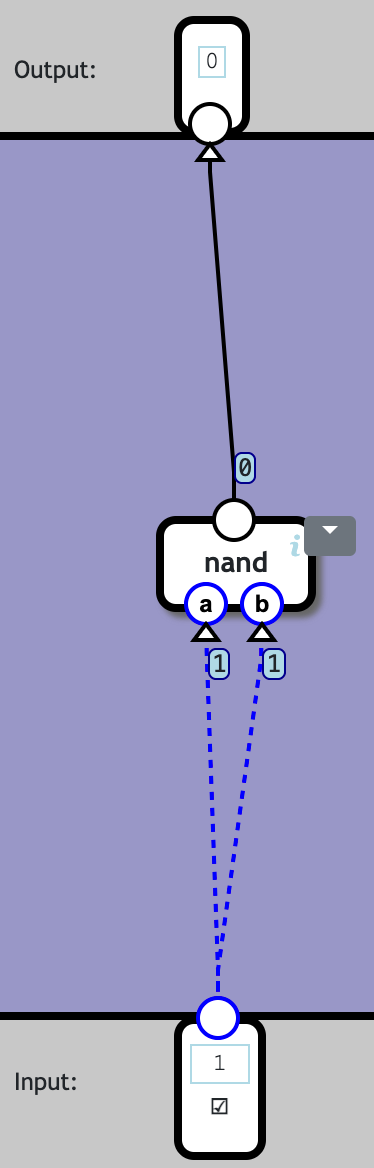
\includegraphics[scale=0.2]{not.png}\par 
			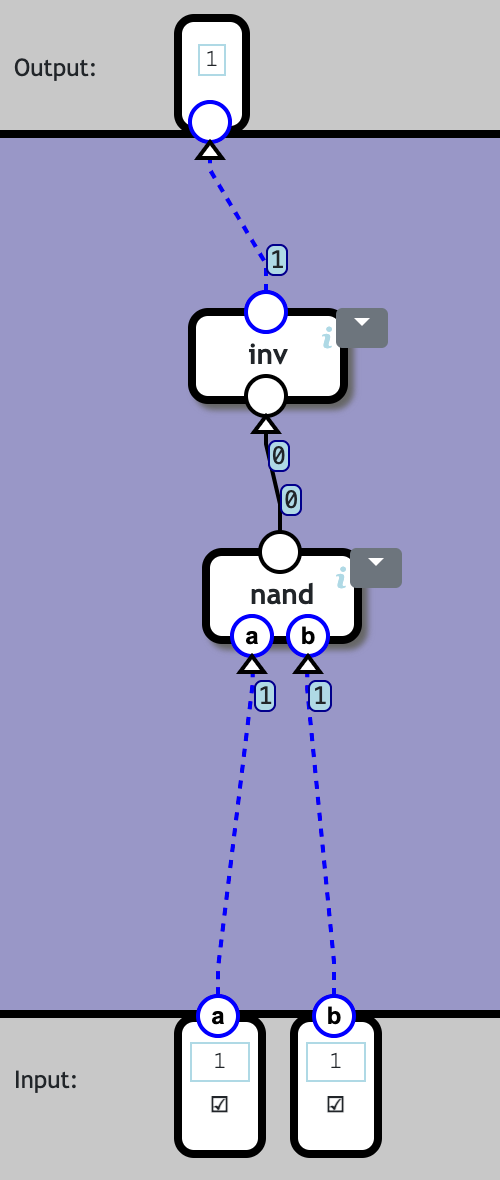
\includegraphics[scale=0.2]{and.png}\par 
				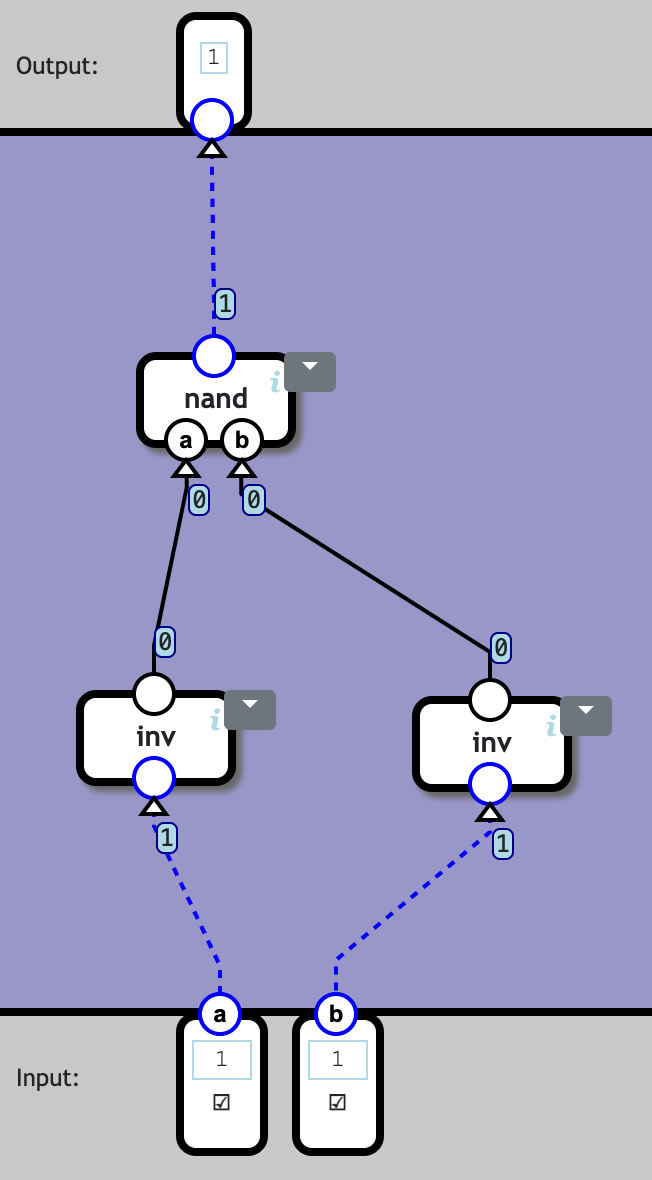
\includegraphics[scale=0.2]{or.png}\par
		\end{multicols}
		\begin{multicols}{3}
		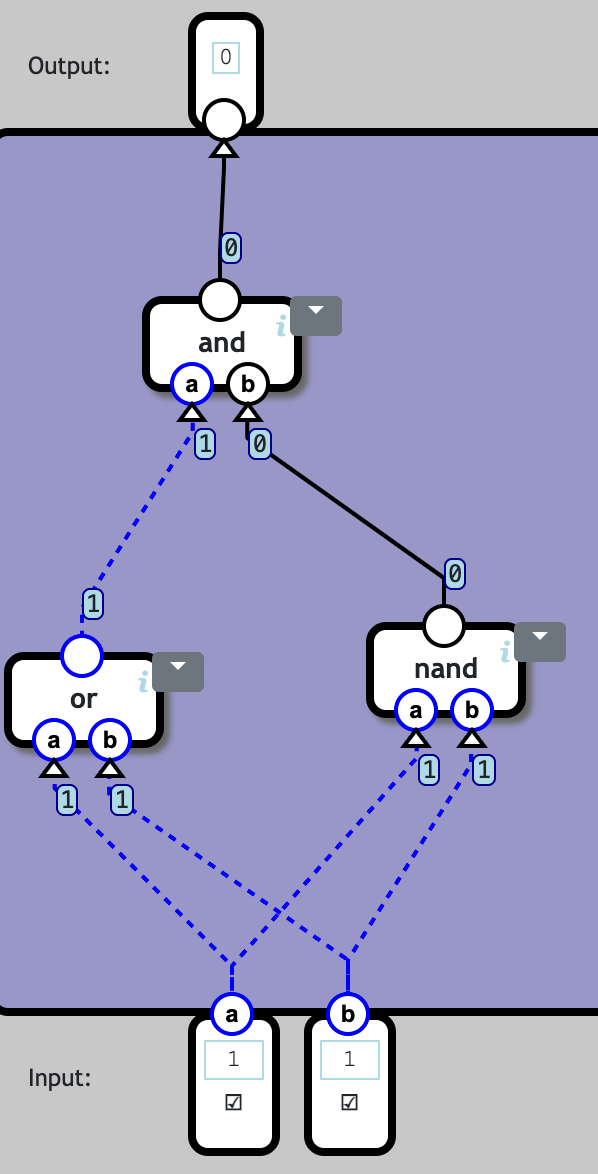
\includegraphics[scale=0.2]{xor.png}\par
				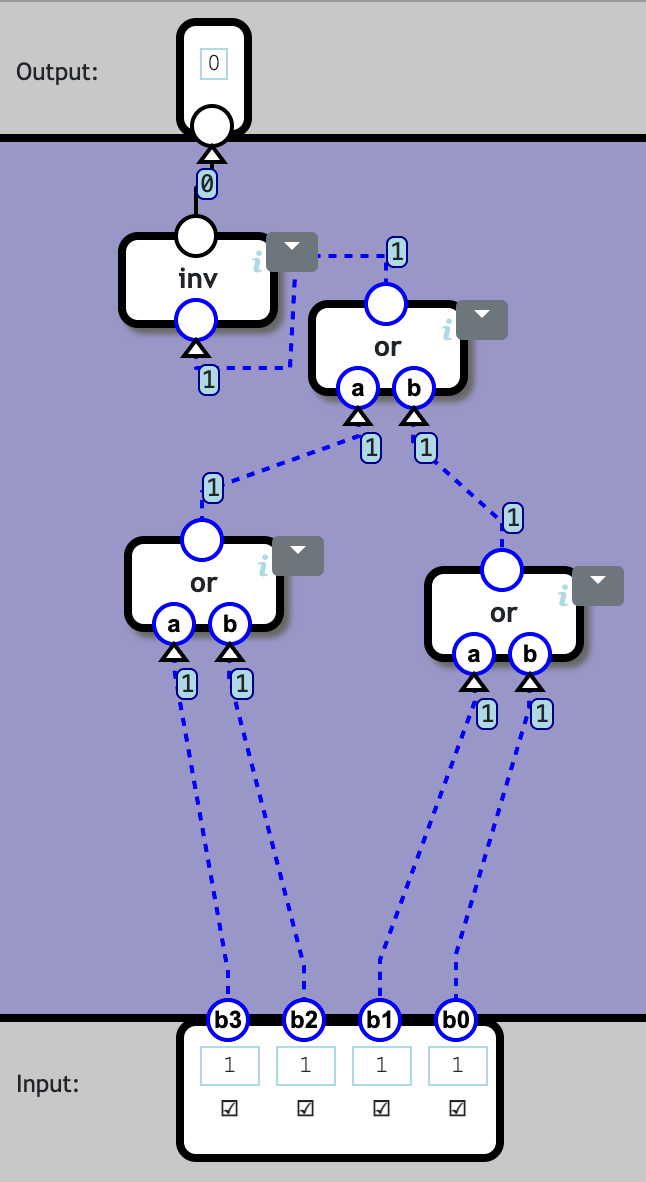
\includegraphics[scale=0.2]{equal-to-zero.png}\par
					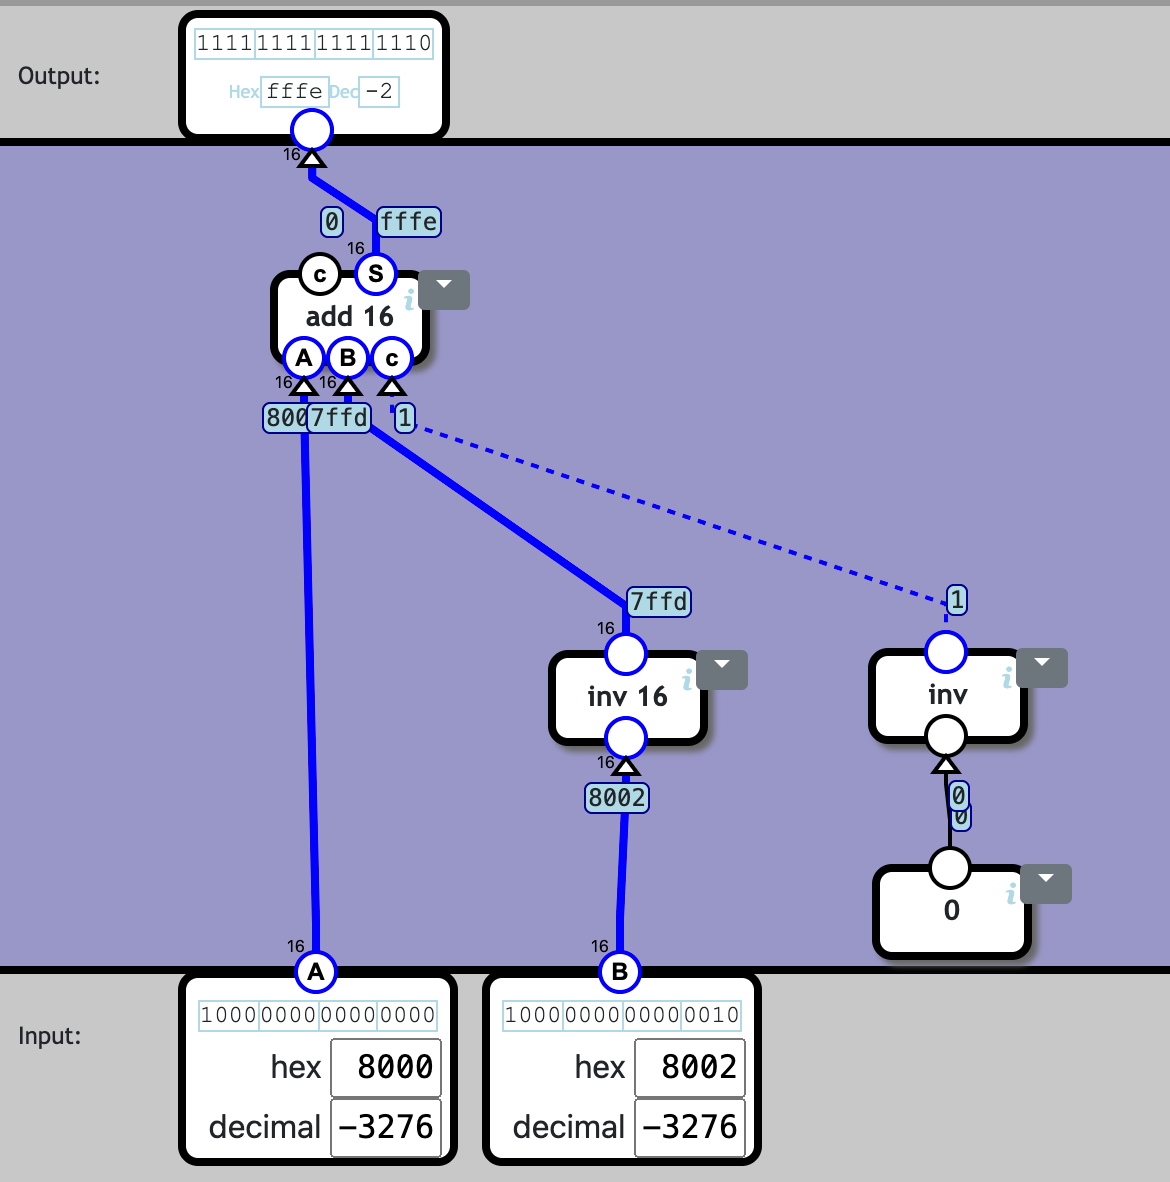
\includegraphics[scale=0.2]{subtractor.png}\par
		\end{multicols}
		\caption{Top row: Not, And, Or implementations. Bottom row: Xor, Equal-to-Zero, Subtractor  }
	\end{figure*}

	\end{enumerate}

\end{document}
